\documentclass[a4paper,11pt]{article}
%\usepackage{ucs}
\usepackage{pstricks}
\usepackage[utf8]{inputenc}
\usepackage{amsmath}
\usepackage{amsfonts}
\usepackage{amssymb}
\usepackage{amsthm}
\usepackage[spanish]{babel}
\usepackage{graphicx}
\usepackage{graphics}
\usepackage[margin=1in]{geometry}
\usepackage{fancyhdr}
%\usepackage{subfigure}
%\usepackage{wrapfig}
%\usepackage[amssymb,mediumspace]{SIunits}
\usepackage{listings}
%\usepackage{fullpage}
\usepackage{color}

\newcommand{\HRule}{\rule{\linewidth}{0.5mm}}
\pagestyle{fancy}
% Title Page
\setlength{\headwidth}{\textwidth}
\fancyhead[L]{TEL-332}% empty left
\fancyhead[R]{Multimedios}

%\renewcommand{\headheight}{0.6in}


% listings

\definecolor{Brown}{cmyk}{0,0.81,1,0.60}
\definecolor{OliveGreen}{cmyk}{0.64,0,0.95,0.40}
\definecolor{CadetBlue}{cmyk}{0.62,0.57,0.23,0}
\definecolor{lightlightgray}{gray}{0.9}

\definecolor{lightgray}{rgb}{.9,.9,.9}
\definecolor{darkgray}{rgb}{.4,.4,.4}
\definecolor{purple}{rgb}{0.65, 0.12, 0.82}

\lstdefinelanguage{JavaScript}{
  keywords={typeof, new, true, false, catch, function, return, null, catch, switch, var, if, in, while, do, else, case, break},
  keywordstyle=\color{OliveGreen}\bfseries,
  ndkeywords={class, export, boolean, throw, implements, import, this},
  ndkeywordstyle=\color{darkgray}\bfseries,
  identifierstyle=\color{black},
  sensitive=false,
  comment=[l]{//},
  morecomment=[s]{/*}{*/},
  commentstyle=\color{CadetBlue}\ttfamily,
  stringstyle=\color{Brown}\ttfamily,
  morestring=[b]',
  morestring=[b]"
}

\lstset{
	language=Python,                             % Code langugage
	basicstyle=\ttfamily,                   % Code font, Examples: \footnotesize, \ttfamily
	keywordstyle=\color{OliveGreen},        % Keywords font ('*' = uppercase)
	commentstyle=\color{gray},              % Comments font
%	numbers=left,                           % Line nums position
%	numberstyle=\tiny,                      % Line-numbers fonts
	stepnumber=1,                           % Step between two line-numbers
	numbersep=5pt,                          % How far are line-numbers from code
	backgroundcolor=\color{lightlightgray}, % Choose background color
	frame=none,                             % A frame around the code
	tabsize=2,                              % Default tab size
	captionpos=b,                           % Caption-position = bottom
	breaklines=true,                        % Automatic line breaking?
	breakatwhitespace=false,                % Automatic breaks only at whitespace?
	showspaces=false,                       % Dont make spaces visible
	showtabs=false,                         % Dont make tabls visible
	columns=flexible,                       % Column format
	showstringspaces=false,
}


\title{Proyecto de multimedios\\Dudo!}
\author{Juan Mucarquer\\2830027-1\\\small{\texttt{<juan.mucarquer@alumnos.usm.cl>}} \and Sebastian Cáceres\\2830010-7\\\small{\texttt{<sebastian.caceresb@alumnos.usm.cl>}} \and Victor Fernandez\\2604041-8\\\small{\texttt{<victor.fernandez@alumnos.usm.cl>}}}
\begin{document}
%\begin{titlepage}
%	\input{portada}
%\end{titlepage}
\maketitle
%\renewcommand\thesubsection{\thesection\alph{subsection}}
%\setcounter{section}{1}

\newpage
\tableofcontents
\newpage

\section{Introducción}
\subsection{Trasfondo}
	En la actualidad, el desarrollo de aplicaciones web es muy popular. 
La mayoría de la gente tiene acceso a internet, y el mercado es muy prometedor.
Existen cientos (o miles) de aplicaciones con distintos fines, muchas muy 
buenas. Otras, quizás no tanto. \\

	Un subconjunto de estas aplicaciones son los juegos online. Estos 
juegos se han vuelto muy populares últimamente, probablemente debido a la
capacidad que poseen para manejar partidas multijugadores.\\

 Esto es muy atractivo, y existe una gran variedad de juegos que disponen 
de esta característica. Sin embargo, por lo general son solo típicos juegos 
de cartas.El enfoque que tomaremos será hacer algo distinto, implementar 
un juego de mesa que no sea de cartas, pero que tenga características 
similares a las descritas anteriormente. \\

El juego que implementaremos será el dudo.  
	

\subsection{Resumen}

	El proyecto descrito en este informe será la implementación de
un juego basado en la  arquitectura cliente-servidor. Este juego será 
el típico juego latinoamericano de especulación, el dudo.\\

	Éste juego será multijugador, de manera de que puedan jugar múltiples 
personas en red, ubicadas en distintos lugares físicos, pero compartiendo el
mismo contexto de la partida. Éstas partidas de desarrollarán en salas de 
juego independientes unas de otras, y cada una tendrá un ganador. \\
	
	Dentro de cada sala habrá un chat para que los usuarios puedan 
comunicarse entre ellos, libremente.
	La implementación también ofrecerá un sistema de usuarios. Para jugar
será necesario registrarse. Por último, la dinámica del juego está regida por 
reglas detalladas en otra sección dentro de este mismo informe 

\newpage
\section{Descripción General}
\subsection{Objetivos}
\subsubsection{General}

	El objetivo principal de la aplicacion es ofrecer una plataforma para
un juego popular chileno, en linea, activo y rapido. La lógica del juego
es de relativa sencillez y las reglas son ampliamente conocidas, por lo que
pretende que el juego sea fácil e intuitivo para el usuario.

 
\subsubsection{Especificos}
\begin{itemize}
	\item Promover el juego del dudo.
	\item Disponer de un juego rapido e instantaneo
	\item Utilizar tecnologías que permitan su jugabilidad de forma nativa,
	no es necesario descargar nada para empezar a jugar.
	\item Contar con un chat y salas de juego.
	\item Establecer un protocolo de comunicación entre el cliente y el servidor (definición de mensajes).
\end{itemize}

\subsection{Problemática que enfrenta}

	La problemática que enfrenta el juego es, por un lado, el aburrimiento de las pobres personas. La gente necesita un juego bien codificado y funcional
que les brinde un alto nivel de entretención.\\

	Por otro lado, si bien existen bastantes juegos online en la actualidad,
creemos que no existe ninguno con el cual el usuario se pueda identificar,
debido a que ninguno de los que existe ahora es propiamente latinoamericano. 

\subsection{Descripción de la solución}
	
	La solución para ambas problemáticas es implementar el dudo 
multijugador online. Éste está dividido en dos partes: el cliente y el servidor.
\\

	En el lado del cliente, existirá un sistema de login, seguido de un 
menú de selección de salas, el cual mostrará las salas disponibles y los 
usuarios que estan en cada sala. El cliente entonces podrá elegir una sala 
para jugar su partida, la cual también contará con un chat en el cual 
participarán los jugadores que compartan una partida.\\

	El servidor se encargará del paso de mensajes asincrónico, y de las
interacciones con la base de datos. Con esto, el servidor definirá la 
estructura del juego, y su secuencia. Esto se refiere a manejo de turnos, 
de interacciones entre usuarios, de mensajes de chat, de usuarios dentro de 
la sala, de dados disponibles por usuario y su aleatorización, etc.
	

\subsection{Tecnologias utilizadas}
Para la parte del servidor, constará de una aplicacion MVC, utilizando el framework
Django (Python). Con el fin de tener una comunicación asincronica y activa entre
el cliente y el servidor, se utilizará un binding de la biblioteca Socket.IO (Javascript),
construido sobre gevent, una biblioteca basadas en co-rutinas para aplicaciones de red, llamado
gevent-socketio. Como Key-value store se utilizó la base de datos NoSQL Redis\\

En el cliente se utilizará HTML5 y CSS para el diseño, y para la comunicación, Javascript
con la biblioteca Socket.IO, basada a su vez en node.js.En específico, para 
 la interfaz gráfica, se utilizará Twitter Bootstrap, la cual es una colección
de herramientas para la creación de diseños web. Contiene platillas HTML y CSS,
y interacciones con javascript para un diseño eficiente. \\

Se posee un repositorio git para el control de versiones, hospedado en 
github.com. Este informe también se encuentra disponible en el repositorio.
Se puede acceder a él mediante el código QR disponible en la portada del 
informe, o accediendo a https://github.com/jamonardo/cacho.

\newpage
\section{Especificación de los requerimientos}
	
	Para especificar los requerimientos, primero es necesario establecer 
las reglas del juego.

\subsection{Reglas del juego}

	El juego parte cuando hay más de un jugador listo para comenzar.
 Cada jugador parte con un total de 5 dados dentro de su \textit{cacho}. Las 
rondas del juego se realizan en sentido antihorario.\\

	Al comienzo de cada \textit{ronda}, los jugadores agitan los dados del 
cacho, es decir, reciben aleatoriamente los valores contenidos en sus dados.
Sólo ellos son capaces de ver el contenido de su cacho, no así los demás. \\

	En base a el contenido de su cacho, cada jugador especula el resultado 
de la suma de todos los dados cara arriba - con un determinado numero - 
obtenidos en total por todos los jugadores. Los ases, aparte de ser números
concretos, con comodines, y pueden obtener el valor del número que se esta 
contando.\\

	El jugador que parte \textit{canta} un número estimado de dados. 
\textbf{(ej: "Hay tres quinas")}. \\

	El jugador siguiente tiene dos opciones: elevar el número especulado,
o dudar. \\

\begin{itemize}
\item Para elevar el número, existen tres maneras posibles. Una es aumentar la 
\textit{"pinta"} del dado (ej: De tres quinas a tres sextas). Otra es aumentar
 el número de dados totales en la especulación (ej: De tres quinas a cuatro 
quinas). La última manera es una combinación de las dos maneras anteriores.
\item Si el jugador duda, todos los jugadores muestran los dados contenidos
en sus cachos, y estos se cuentan. Si la especulación era correcta, es decir,
hay sobre la mesa el número total de dados cantados por el primer jugador, el 
jugador que dudó pierde un dado. En el caso contrario, el jugador que cantó,
pierde un dado.
\end{itemize}

	El jugador que comienza cantando la siguiente ronda es el que pierde.\\

	Cuando a un jugador le queda un sólo dado, el jugador \textbf{obliga}.
En este caso, y sólo para esta ronda, sólo él puede ver el contenido de su 
cacho, nadie mas. Una vez que el jugador cante, nadie puede cambiar la pinta
cantada, y los ases dejan de ser comodines.\\

	El juego se termina cuando sólo queda un jugador con dados en su cacho,
y es él quien gana.\\

%\newpage

\subsection{Usuarios del sistema}

\begin{description}
	\item[Administrador] \hfill \\ \\
	El administrador es el encargado de crear y 
	regular los espacios y las características de la sala. Dentro de estos
	se incluyen la creación de salas, usuarios, etc.

	\item[Clientes] \hfill \\ \\
	Serán los principales usuarios del sistema. Los 
	clientes acceden al sistema, seleccionan salas, y juegan partidas.
\end{description}
\newpage	

\subsection{Descripción de los requerimientos}
\subsubsection{Funcionales}

\begin{description}
	\item[Requisito 1] \hfill \\ \\
	Implementar login y registro de usuarios.
	\item[Requisito 2] \hfill \\ \\
	Implementar login y panel de control de administrador.
	\item[Requisito 3] \hfill \\ \\
	Lista de salas de juego disponibles.
	\item[Requisito 4] \hfill \\ \\
	Lista de usuarios dentro de salas de juego.
	\item[Requisito 5] \hfill \\ \\
	Chat dentro de la sala de juego.
	\item[Requisito 6] \hfill \\ \\
	Botón confirmar inicio del juego, el cual es necesario que pulsen
	todos los jugadores dentro de una sala para comenzar la partida.
	\item[Requisito 7] \hfill \\ \\
	Implementación de lógica de juego del lado del servidor.
	\item[Requisito 8] \hfill \\ \\
	Display con dados disponibles por usuario, y dados obtenidos en cada 
	turno.
	\item[Requisito 9] \hfill \\ \\
	Determinar el ganador de la partida, y boton de salida de la sala
	dinámico, el cual aparece una vez que la partida termine.
	\item[Requisito 10] \hfill \\ \\
	Display que diga quien está jugando actualmente.
\end{description}
%\newpage

\subsubsection{No funcionales}

\begin{description}
	\item[Sencillez de uso] \hfill \\ \\
	El uso del sistema y de sus componentes debe ser intuitivo, lo mas 
	sencillo posible. Las opciones para el usuario deben estar acordes
	a estos principios.
	Para esto, se diseñará la interfaz gráfica de la manera mas sencilla
	que se pueda, no utilizando interacciones complejas, y haciendo
	que las opciones disponibles lo más evidentes y sencillas posibles. 
	\item[Fluidez] \hfill \\ \\
	Por otra parte, el juego debe funcionar lo más fluidamente posible.
	Esto significa que toda la interacción del usuario, desde su login, 
	mientras dure la partida y su finalización, deben transcurrir dentro 
	de lo posible sin retardos ni cortes.
	Para esto, se utilizará gevent-socketio, enfatizando que las 
	interacciones con dependencia de otros componentes
	sean lo más breves posibles, de manera que los tiempos de respuesta
	sean mínimos. 
	\item[Escalabilidad] \hfill \\ \\
	El sistema debe ser modular en su construcción, permitiendo así 
	añadir futuras funcionalidades al juego que puedan mejorar su
	calidad. Es importante que se pueda hacer esto sin afectar la 
	codificación hecha anteriormente.
	Para esto, se diseñará modularmente, haciendo que cada parte del código
	sea un módulo, y permitiendo la posibilidad de integrar varios más
	en el caso de que se desee agregar mas componentes.

\end{description}
\newpage

\subsection{Tareas de usuario}

\begin{description}
	\item[Administrador] \hfill \\ \\
	La tarea del administrador es velar por el correcto orden esquemático
	del sitio. El estará encargado de crear salas, administrarlas o 
	borrarlas, dependiendo del caso. También tiene las mismas 
	responsabilidades con respecto a los usuarios. Al final de cuentas,
	es un usuario que interactúa directamente con la base de datos.

	\item[Clientes] \hfill \\ \\
	La tarea principal (y única) de los clientes será jugar partidas. Ellos
	ingresarán a el juego, logeandose. Luego buscarán una sala disponible.
	Al ingresar a una sala disponible, podrán salirse de ella, o confirmar
	su participación para el inicio del juego. Una vez terminada la partida,
	el usuario se sale de la sala, y vuelve a escoger otra sala disponible
	para jugar, o derechamente se sale del sistema.
	
\end{description}
\newpage
	

\subsection{Funciones del sistema}
Las funciones del sistema serán:\\

\textbf{Servidor:}
\begin{itemize}
	\item Manejar las sesiones de los usuarios, entrando
	mediante un formulario de login y permitir el registro de usuarios,
	usando un formulario de registro.
	\item Derivar las peticiones hechas por HTTP a la vista
	correspondiente (urls.py)
	\item Formatear la informacion para cada vista.
	\item Mostrar una lista de salas de juego con los usuarios
	dentro de cada sala y el estado de la sala (jugando o esperando).
	\item Derivar las conexiones y mensajes hechas mediante el 
	protocolo de Socket.IO hacia un modulo que se encargará de responder
	a estos mensajes (cacho\_socketio.py)
	\item Inicializar y responder a los mensajes enviados por los clientes,
	según un protocolo de juego, descrito posteriormente en el 
	diagrama de secuencia.
	\item Mantener e interactuar con el modelo de datos para las
	operaciones que lo requieran.
\end{itemize}
\vspace{0.7cm}
\textbf{Cliente:}
\begin{itemize}
	\item Registrarse con un nombre de usuario y contraseña
	\item Unirse a una sala de juego que actualmente esté esperando
	jugadores.
	\item Enviar un mensaje a una sala de juego
	\item Confirmar el inicio del juego por parte de un usuario.
	\item Recibir y mostrar los dados para el jugador
	\item Enviar una jugada, un dudo o calzo.
	\item Salir de la sala una vez terminada la partida.
\end{itemize}
\newpage

\section{Diseño de la interfaz de usuario}
\subsection{Esquema navegacional}
\begin{figure}[h]
	\centering
	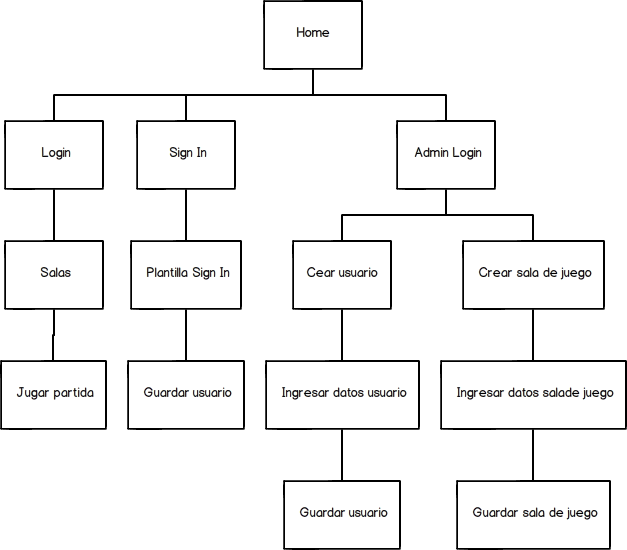
\includegraphics[width=\textwidth]{Esquema_navegacional.png}
\end{figure}
\newpage

\subsection{Vistas}
\begin{figure}[h!]
	\centering
	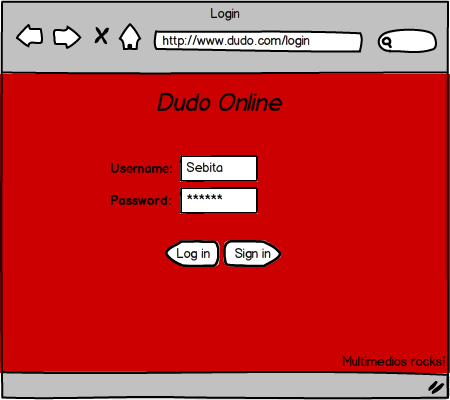
\includegraphics[width=0.9\textwidth]{Login.png}
	\caption{Login}
\end{figure}

\begin{figure}[h!]
	\centering
	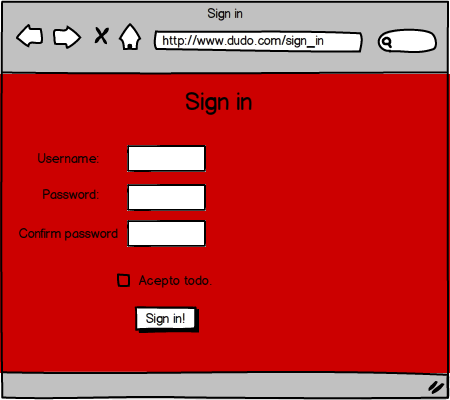
\includegraphics[width=0.9\textwidth]{Sign_in.png}
	\caption{Sign in}
\end{figure}
\newpage
\begin{figure}[h!]
	\centering
	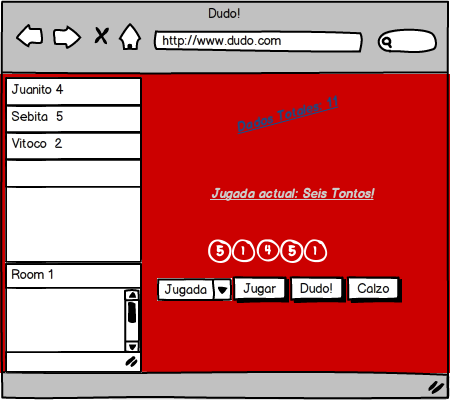
\includegraphics[width=0.9\textwidth]{Sala.png}
	\caption{Sala de juego}
\end{figure}

\begin{figure}[h!]
	\centering
	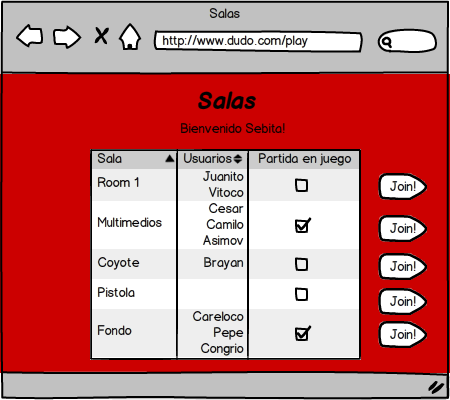
\includegraphics[width=0.9\textwidth]{salas.png}
	\caption{Lista de salas de juego}
\end{figure}
\newpage
\begin{figure}[h!]
	\centering
	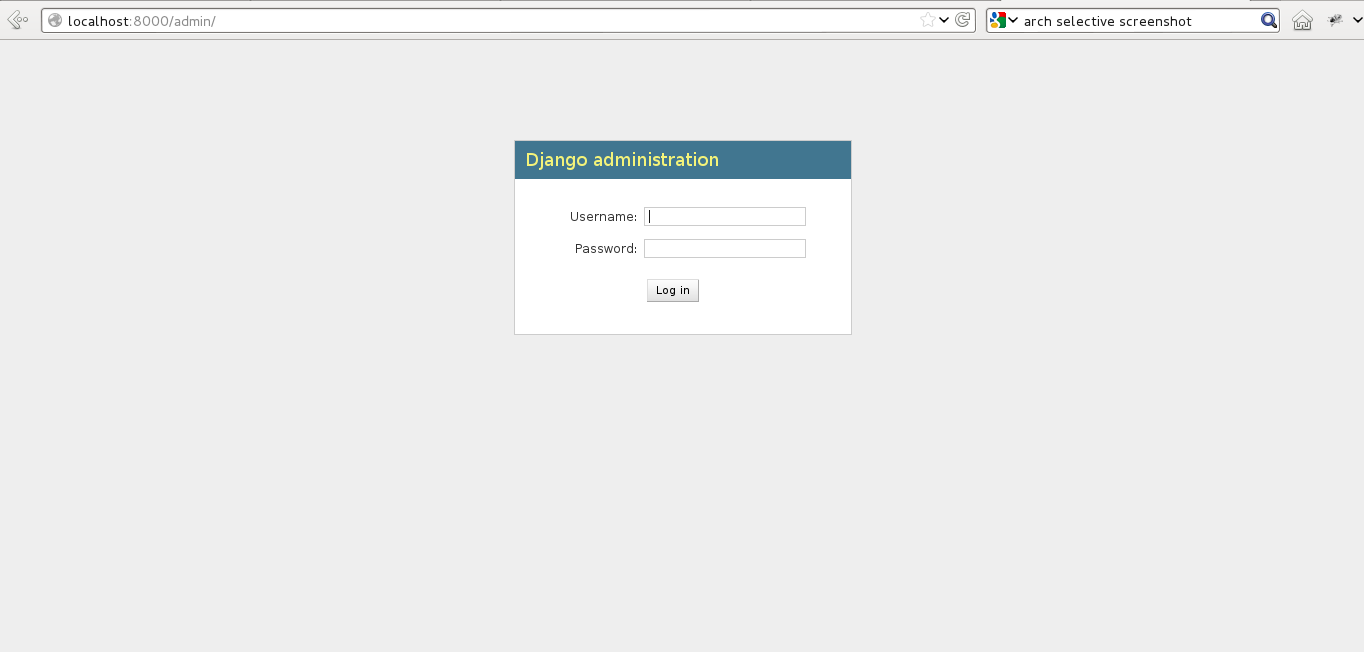
\includegraphics[width=0.9\textwidth]{Admin_log.png}
	\caption{Log in del panel de administración}
\end{figure}

\begin{figure}[h!]
	\centering
	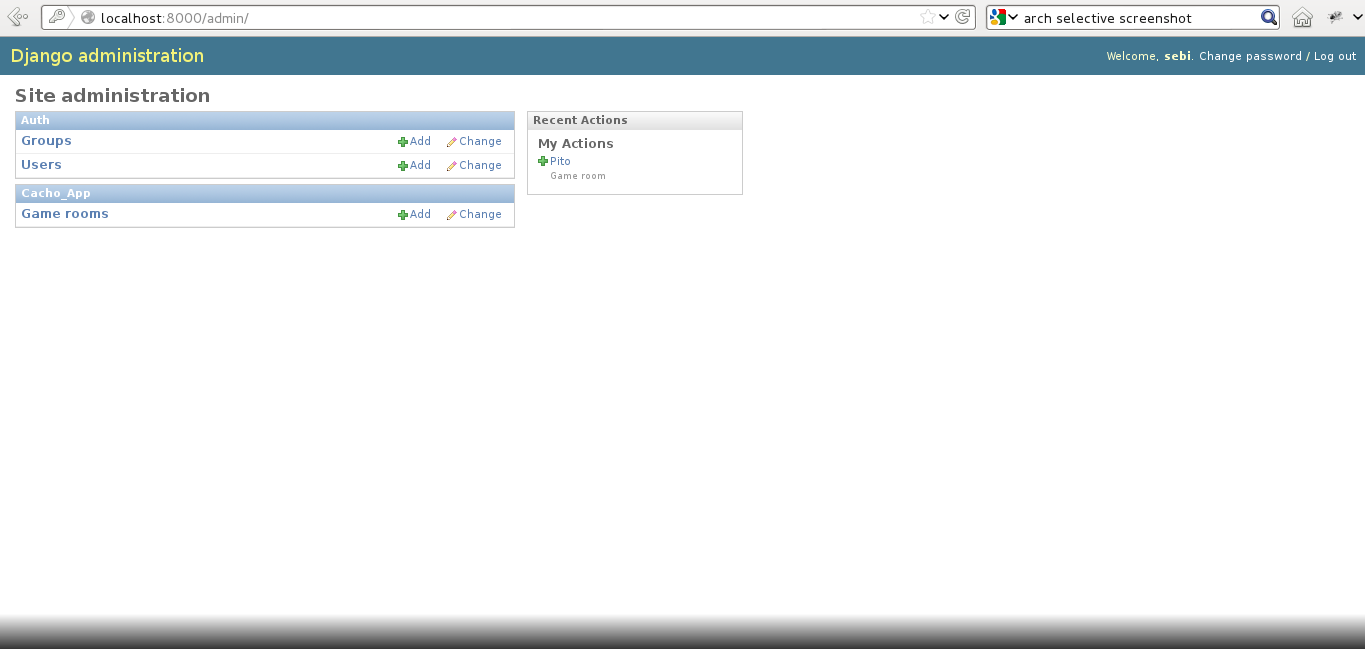
\includegraphics[width=0.9\textwidth]{AdminCp.png}
	\caption{Vista principal del panel de administración}
\end{figure}

\begin{figure}[h!]
	\centering
	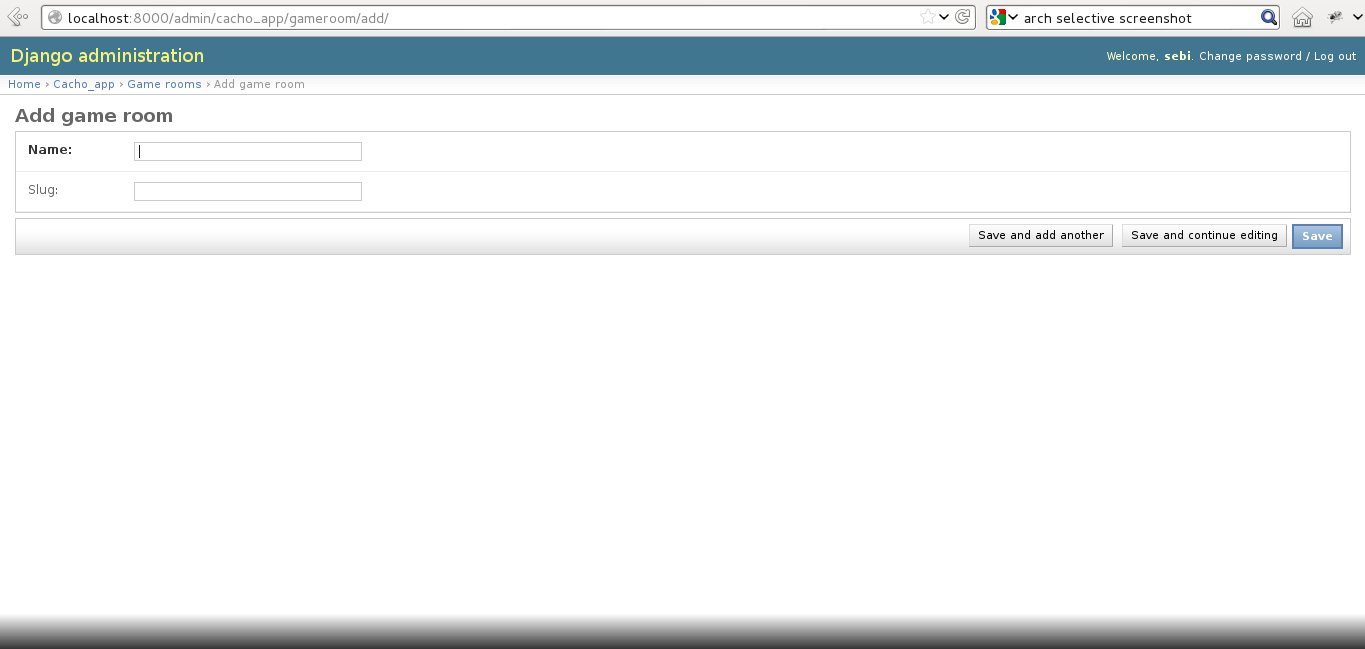
\includegraphics[width=0.9\textwidth]{Admin_addroom.png}
	\caption{Agregar nueva sala}
\end{figure}

\begin{figure}[h!]
	\centering
	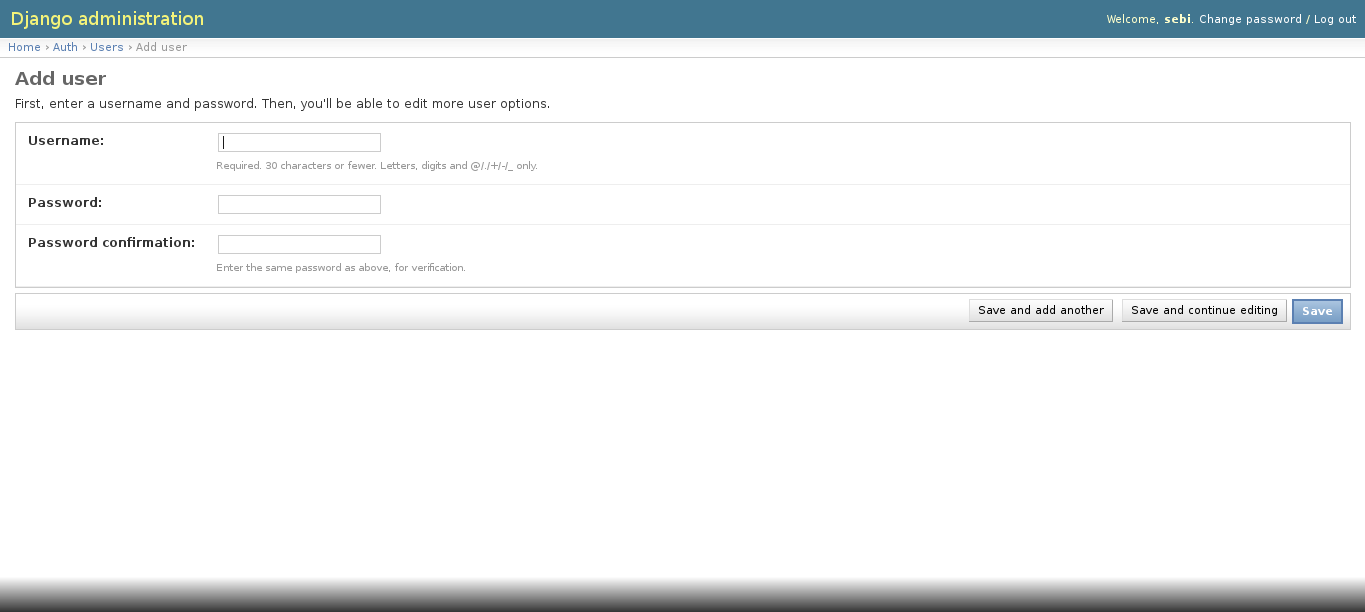
\includegraphics[width=0.9\textwidth]{Admin_adduser.png}
	\caption{Agregar nuevo usuario}
\end{figure}

\begin{figure}[h!]
	\centering
	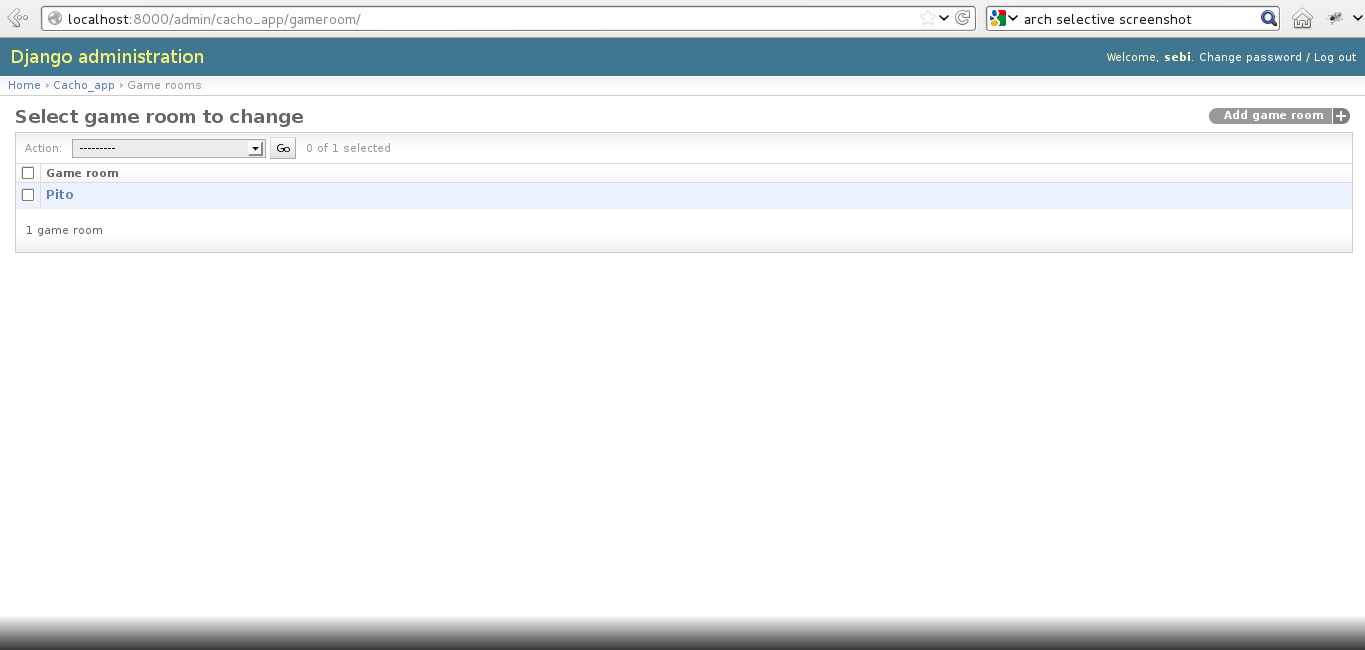
\includegraphics[width=0.9\textwidth]{Admin_room_cp.png}
	\caption{Editar sala}
\end{figure}
\begin{figure}[h!]
	\centering
	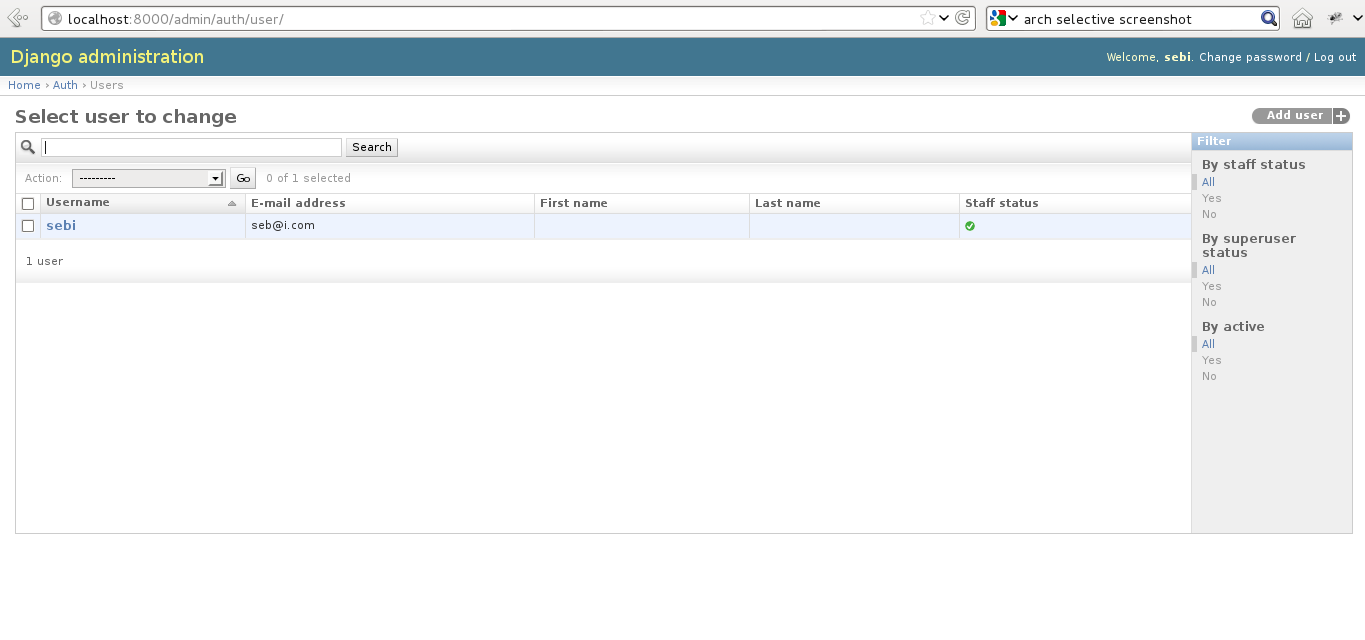
\includegraphics[width=0.9\textwidth]{Admin_user_cp.png}
	\caption{Editar usuario}
\end{figure}

\newpage

\section{Diseño del sistema}
\subsection{Diseño de la arquitectura}
	El diseño de arquitecturas que utilizaremos será el modelo MVC. 
Este se divide en 3 partes:
\begin{itemize}
	\item \textbf{Modelo:} El modelo es una entidad que representa la 
información específica con la cual el sistema opera (La base de datos). 
Interactúa con la \textbf{Vista} y el \textbf{Controlador} cuando hay un cambio
de su estado. Esta interacción permite a la vista entregar contenido actualizado, 
y a el controlador a cambiar el set de comandos disponibles. \\
	\item \textbf{Controlador:} El controlador maneja el modelo, 
interactúa con él y lo modifica, en respuesta a  eventos generados por el 
usuario. El controlador también puede interactuar con las vistas, 
actualizandolas. \\
	\item \textbf{Vista:} La vista interactúa con el modelo, pidiendole la
información que necesita para representar los datos para el usuario. \\
\end{itemize}

Elegimos esta arquitectura porque resulta natural trabajar con ella 
para el tipo de proyecto que estamos desarrollando. La mayoría del 
funcionamiento del sistema esta basado en eventos que van a gatillar 
interacciones con el modelo, y estas modificaciones del mismo producirán 
cambios en la vista, ocurriendo todo esto asincrónicamente.
\newpage
\subsection{Diseño lógico}
%\subsubsection{Diagrama de clases}
\subsubsection{Diagrama de casos de uso}
	El diagrama de casos de uso presenta a los dos actores presentes en
el juego: el cliente y el administrador. En el se especifican las funciones e
interacciones que tienen cada uno de ellos con el sistema.
\begin{figure}[h!]
	\centering
	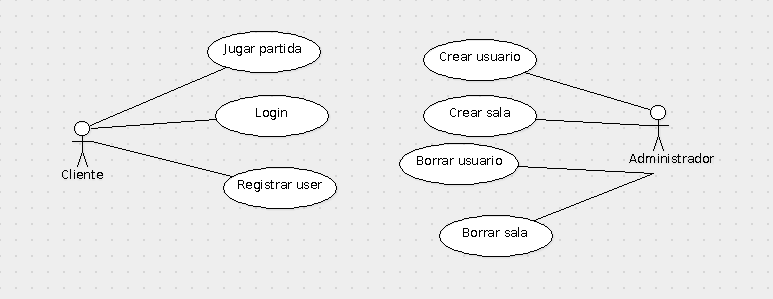
\includegraphics[width=0.9\textwidth]{diag_casos_uso.png}
\end{figure}

\subsubsection{Modelo de datos}
El modelo de datos se adjunta en el apendice. Solo fué necesaria la creacion de \texttt{GameRoom}

\newpage
\subsubsection{Diagrama de secuencia}
El siguiente diagrama de secuencia muestra el protocolo de intercambio de mensajes
entre el cliente y el servidor para un juego. Mas adelante se explicará el contexto
y el significado de cada mensaje.
\begin{figure}[h!]
	\centering
	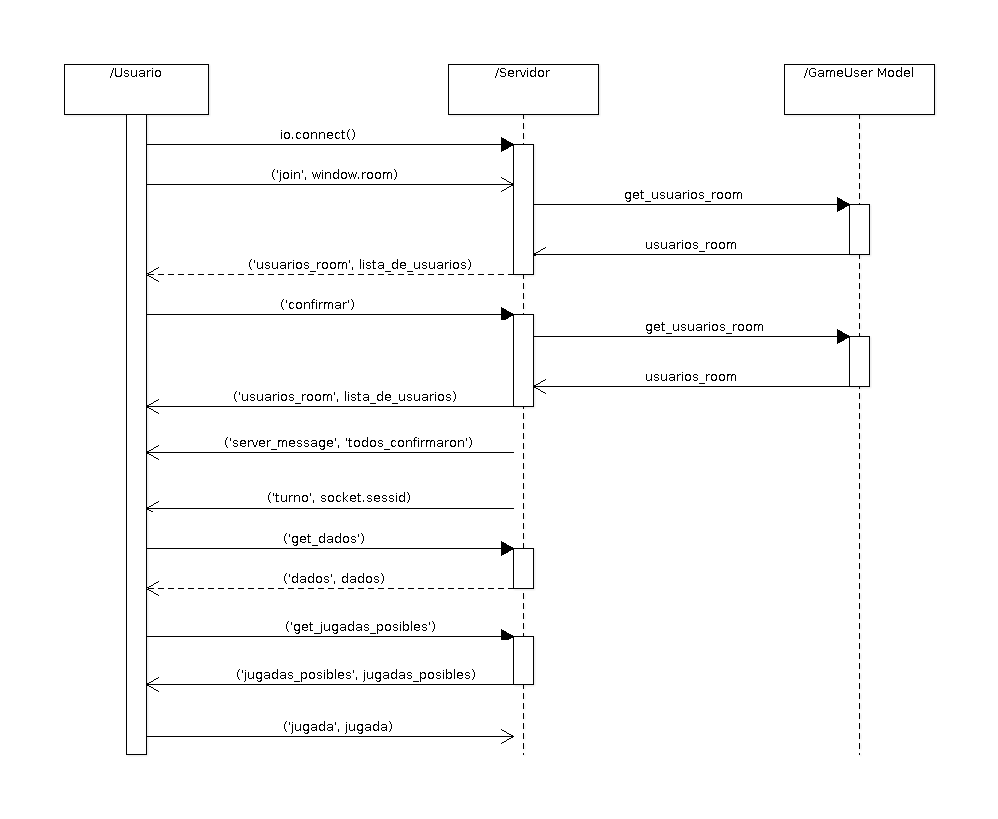
\includegraphics[width=\textwidth]{seq_juego.png}
\end{figure}

\subsubsection{Diagrama de flujo de la lógica del juego}
El diagrama de flujo adjunto en el apendice muestra como se desarrolla el juego una vez
que a un jugador le llega un turno. Esto se ejecuta desde el inicio por cada
turno jugado.

\newpage
\section{Implementación}
\subsection{Descripción de componentes}
Actualmente, el servidor consta de un proyecto de Django, el cual tiene dos aplicaciones,
\texttt{cacho\_site} y \texttt{cacho\_app}.\\

\texttt{cacho\_site} contiene objetos y sistemas
relacionados con el sitio entero, se compone de los siguientes modulos:\\

\textbf{urls.py:} Derivará una URL hacia una vista o módulo.
En el caso de \texttt{/socket.io}, lo derivará al Namespace especifico
al cual se quiere conectar. Al ingresar a \texttt{/play/} se cargarán las URL
de la aplicación \texttt{cacho\_app}.
\begin{lstlisting}[language=Python, caption=cacho\_site/urls.py]
urlpatterns = patterns('',
	url(r'^admin/', include(admin.site.urls)),
	url(r'^login/$', 'django.contrib.auth.views.login'),
	url(r'^play/', include("cacho_app.urls")),

	# socket.io
   url("^socket\.io", include(socketio.sdjango.urls)),
)

urlpatterns += patterns('cacho_site.views', 
	# login logout
	url(r'^logout/', 'logout_view'),
\end{lstlisting}
\vspace{1cm}
\textbf{views.py}: Renderizará un template para el index y hará el logout.
El objeto \texttt{request.user} mantiene las variables de sesion del usuario logueado.
\texttt{@login\_required} es un decorador de la aplicación de autenticacion que provee
Django (\texttt{django.contrib.auth}), un filtro para usar el metodo que le sigue.
\begin{lstlisting}[language=Python, caption=cacho\_site/views.py]
@login_required
def index(request):
	context = {"user": request.user}
	return render(request, 'index.html', context)
\end{lstlisting}

\newpage
\subsection{Aplicación del juego}
\texttt{cacho\_app} pretende mantener objetos y módulos relacionados solo
con la aplicación de juego, usando las sesiones y modelos de \texttt{cacho\_site}.\\

Se compone de los siguientes modulos:\\

\textbf{urls.py}: Cuando se ingresa a \texttt{/} (\texttt{/play/}) se mostrará
la lista de las salas, mientras que por un nombre, se ingresará a la sala con el
\texttt{slug} de la URL.
\begin{lstlisting}[caption=cacho\_app/urls.py]
urlpatterns = patterns("cacho_app.views",
	url("^$", "rooms", name="rooms"),
	url("^(?P<slug>.*)$", "room", name="room"),
)
\end{lstlisting}
\vspace{1cm}
\textbf{views.py}: Dos vistas, una para listar todos los rooms, haciendo
referencia al modelo (GameRoom) y luego renderizando la vista mediante el template
\texttt{rooms.html}. \texttt{room} buscará el slug en el modelo y lo enviará al template
para renderizarlo. Si no encuentra el slug arrojará un error 404.
\begin{lstlisting}[caption=cacho\_app/views.py]
@login_required
def rooms(request, template="rooms.html"):
    """
    Listar todos los rooms y sus participantes
    """
    context = {"rooms": GameRoom.objects.all()}
    return render(request, template, context)

@login_required
def room(request, slug, template="room.html"):
    """
    Entrar a una sala de juego
    """
    logged_user = request.user.get_full_name()
    context = {"room": get_object_or_404(GameRoom, slug=slug), "user": logged_user}
    return render(request, template, context)
\end{lstlisting}
\newpage
\textbf{Dudo.py}: Contiene funciones utilitarias para la logica del juego.
RingBuffer es usado para el manejo de turnos, es una lista circular, la cual a traves
del metodo \texttt{get()} se obtiene el proximo elemento de la lista.\\

Dudo es una clase que implementa un solo metodo hasta el momento, \texttt{posibles(mov, max\_dados)}, donde \texttt{mov} es una 2-tupla que indicará un movimiento. Este metodo devolverá
los movimientos (2-tuplas) que son posibles de realizar (y que van con las reglas del dudo), segun una cantidad de dados. Así, cuando al jugador le llegue el turno, se le enviará una lista de movimientos posibles en base al movimiento efectuado por el jugador anterior. Con esta lista se pretende poblar un formulario en el cliente que tiene el turno, limitando sus jugadas a jugadas que sean posibles y tengan sentido.
\begin{lstlisting}[caption=Dudo.py]
class RingBuffer:
	def __init__(self):
		pass
		
	def remove(self, key):
		pass
		
	def length(self):
		pass
		
	def append(self,x):
		pass
		
	def get(self):
		pass
		
	def get_current(self):
		pass
		
	def previous(self):
		pass
		
	def set(self, x):
		pass
		
class Dudo:
	def posibles(self, movimiento, maximo_dados):
		pass
\end{lstlisting}

\newpage
\textbf{cacho\_socketio.py}: A este módulo llegarán las conexiones y mensajes que 
provienen del cliente Javascript. Según el protocolo de Socket.IO, el cliente 
se debe conectar a un Namespace, un espacio de nombres especifico que mantiene 
un conjunto de funciones (event handlers). En este caso, se definió el namespace 
\texttt{/game}, el cual agrupa eventos referentes al juego. \\

Cada petición \texttt{HTTP GET} será una instancia de esta clase (GameNamespace), por lo tanto
manejará la interacción con un solo cliente logeado. Cada una de estas funciones se ejecutará
dependiendo del mensaje que envíe el cliente. El objeto \texttt{request} al cual se tenía
acceso en \texttt{views.py} es duplicado, y accesible desde aqui como \texttt{self.request},
pudiendo manejar variables de sesión del sitio en el ambiente que interactua con el cliente Javascript.\\

Un mensaje/evento se compone de un nombre y sus datos, los cuales serán serializados a JSON
para su posterior entendimiento en el cliente Javascript. Un metodo del Namespace es el nombre de un evento, precedido por \textbf{on\_}. e.g: el mensaje enviado desde 
el cliente \texttt{('join', room)}, gatillará el evento \texttt{on\_join(self, room\_in)}, donde el argumento será su dato. Este dato como se dijo, puede ser cualquier objeto notado en JSON.\\

Este Namespace hereda metodos y variables que son útiles para la comunicacion: 
\texttt{emit()}, \texttt{emit\_to\_room()}, \texttt{socket.sessid}, por ejemplo. Para una completa lista revisar la API de referencia \footnote{\texttt{https://gevent-socketio.readthedocs.org/en/latest/namespace.html}}

\begin{lstlisting}[caption=cacho\_app/cacho\_socketio.py]
from socketio.namespace import BaseNamespace
from socketio.mixins import RoomsMixin, BroadcastMixin
from socketio.sdjango import namespace

@namespace('/game')
class GameNamespace(BaseNamespace, RoomsMixin, BroadcastMixin):
	def initialize(self):
		pass

	def on_join(self, room_in):
		pass

	def on_confirmar(self, action):
		pass
	
	def on_get_dados(self):
		pass

	def on_get_jugadas_posibles(self):
		pass

	def on_jugada(self, jugada):
		pass
		
	...
\end{lstlisting}
\newpage
\subsubsection{NoSQL Redis}
Para el almacenamiento de datos de una partida (dados y usuarios actuales en una partida) se usó una base de datos Redis\footnote{http://redis.io/} (NoSQL),
el cual almacena en la memoria ram un par de datos (Key-value store).\\

Redis provee comandos para setear y obtener una campo segun su key, los campos utilizados acá fueron strings serializados en JSON, con
el fin de guardar información formateada. Mas información acerca del formato se puede encontrar en los comentarios de
\texttt{cacho\_socketio.py}, método \texttt{on\_join}.\\

\texttt{redis-py}\footnote{https://github.com/andymccurdy/redis-py} es un cliente para Python para los comandos de Redis.
Se implementó el modulo \texttt{redisutils.py}, el cual inicia la conexion al servidor de Redis y contiene funciones útiles para
varios metodos/modulos.

\begin{lstlisting}[caption=cacho\_app/redisutils.py]
redisdb = redis.StrictRedis(host='localhost', port=6379, db=0)

def get_members_info(room):
	members = []
	room_members = list(redisdb.smembers('room_' + room))

	for sessid in room_members:
		members.append(json.loads(redisdb.get('user_' + sessid)))

	return members

def get_members(room):
	return len(redisdb.smembers('room_' + str(room)))

def get_members_name(room):
	members = []
	if get_members(room) == 0:
		return members
		
	room_members = list(redisdb.smembers('room_' + str(room)))
	
	for sessid in room_members:
		members.append(json.loads(redisdb.get('user_' + sessid))['user_name'])
	
	return members
\end{lstlisting}
\newpage
\subsubsection{Modelo de datos}
El modelo de datos se definió en models.py como sigue. La funcion \texttt{slugify} convierte un nombre
que puede contener espacios y otros caracteres en un string que puede ser concatenado a una URL, ese será
el metodo de acceso a una sala.\\


\begin{lstlisting}[caption=cacho\_app/models.py]
class GameRoom(models.Model):

    name = models.CharField(max_length=20)
    slug = models.SlugField(blank=True)
    state = models.BooleanField(default=False) 

    class Meta:
        ordering = ("name",)

    def __unicode__(self):
        return self.name

    @models.permalink
    def get_absolute_url(self):
        return ("room", (self.slug,))

    def save(self, *args, **kwargs):
        if not self.slug:
            self.slug = slugify(self.name)
        super(GameRoom, self).save(*args, **kwargs)

\end{lstlisting}

\newpage
\subsection{Cliente Javascript}
La parte del cliente se compone de los templates
de cada pagina HTML, junto a las hojas de estilo (CSS)
y scripts JS. Estos archivos se ubican en las carpetas
\texttt{templates} y \texttt{static} respectivamente. \\

En una sala de juego, se carga la biblioteca Socket.IO
(\texttt{socket.io.js}), sobre la cual se construiran manipuladores de eventos asincronicos de emisión y recepción de mensajes con el servidor.\\

Al gatillarse estos eventos, irán a producir cambios en el HTML (GUI),
ocupando la biblioteca JQuery para mayor facilidad.\\

El siguiente codigo muestra la implementacion (reducida) del cliente. Considerar lo siguiente:
\begin{itemize}
	\item \texttt{io.connect('/game');} conectará el cliente Socket.IO al \texttt{Namespace}
	\texttt{game}, definido anteriormente en \texttt{cacho\_socketio.py}
	\item \texttt{socket.on('connect', function (username) ...} manipulará la llegada del evento
	\texttt{connect}, con argumento \texttt{username}, luego enviará la peticion a unirse a la sala
	mediante \texttt{emit}
	\item \texttt{socket.on('usuarios\_room', ...} manipulará la llegada del evento \texttt{usuarios\_room}, la cual contendrá como argumento a una lista de usuarios con informacion acerca de ellos en JSON.
	\item En sintesis, el metodo \texttt{emit(event\_name, args)} enviará al servidor el evento \texttt{event\_name},
	conteniendo como información a \texttt{args}. El metodo \texttt{on(event\_name, callback)} ejecutará
	la funcion \texttt{callback} (con argumentos si es que posee mensaje) en la llegada del evento \texttt{event\_name}.
\end{itemize}

\begin{lstlisting}[language=JavaScript, caption=cacho\_app/static/js/cacho.js]
// socket.io specific code
// funciones de socket del cliente.
var socket = io.connect("/game");
var sessid;
var user_list;

var numeros = ['ningun', 'un', 'dos', 'tres', 'cuatro', 'cinco',
					'seis', 'siete', 'ocho', 'nueve', 'diez', 'once',
					'doce', 'trece', 'catorce', 'quince', 'dieciseis',
					'diecisiete', 'dieciocho', 'diecinueve', 'veinte']
var pintas = ['0', 'aces', 'tontos', 'trenes', 'cuartas', 'quintas', 'sextas']

socket.on('connect', function (username) {
   $('#chat').addClass('connected');
   socket.emit('join', window.room);
});

socket.on('user_sessid', function(id) { sessid = id; });
socket.on('turno', function(turno) { ... });
socket.on('usuarios_room', function (usernames) { ... });
...
\end{lstlisting}




\subsection{Notas}
\begin{itemize}
	\item Se usó como base el framework Bootstrap\footnote{http://twitter.github.com/bootstrap/}
	\item Más información técnica acerca de la implementación puede ser encontrada en los comentarios del codigo.
\end{itemize}
\section{Conclusiones}

	Al finalizar el desarrollo de la aplicación, se ha concluido que:

\begin{itemize}
	\item Las funcionalidades del servidor están completas a cabalidad.
	El cliente es completamente funcional al momento de la entrega.
	Se puede seguir escalando su funcionamiento, para aplicar distintas
	opciones, pero para efectos del trabajo asignado, esta terminado.
	\item Diseñar un juego es un proceso muy complicado, y muy extenso.
	La cantidad de componentes que se le pueden agregar son innumerables,
	por lo que es vital programar dejando espacio para futuras 
	modificaciones, mejoras, y elementos nuevos. La escalabilidad es
	necesaria completamente. 
	\item Es muy importante para este tipo de desarrollo el proceso 
	de testing. Dado que es un juego, existen muchísimas interacciones 
	distintas entre los jugadores, dando lugar a muchas instancias que 
	pueden no haber sido previstas por los programadores. En éstas, pueden 
	ocurrir errores, o "bugs", que alteren el curso normal del juego.
	El proceso debe realizarse con el fin de encontrar la mayor cantidad
	de errores posibles antes de sacar al producto de la fase de desarrollo.
 	\item El modelo MVC es muy útil y eficiente a la hora de realizar
	aplicaciones con paso de mensajes asincrónicos, ya que para efectos
	de visualización por parte del cliente, las vistas se actualizan 
	al haber un cambio en el modelo. Resulta muy natural.

\end{itemize}
\newpage 
\appendix
\section{Figuras}

\begin{figure}[h!]
\caption{Diagrama de flujo del juego}
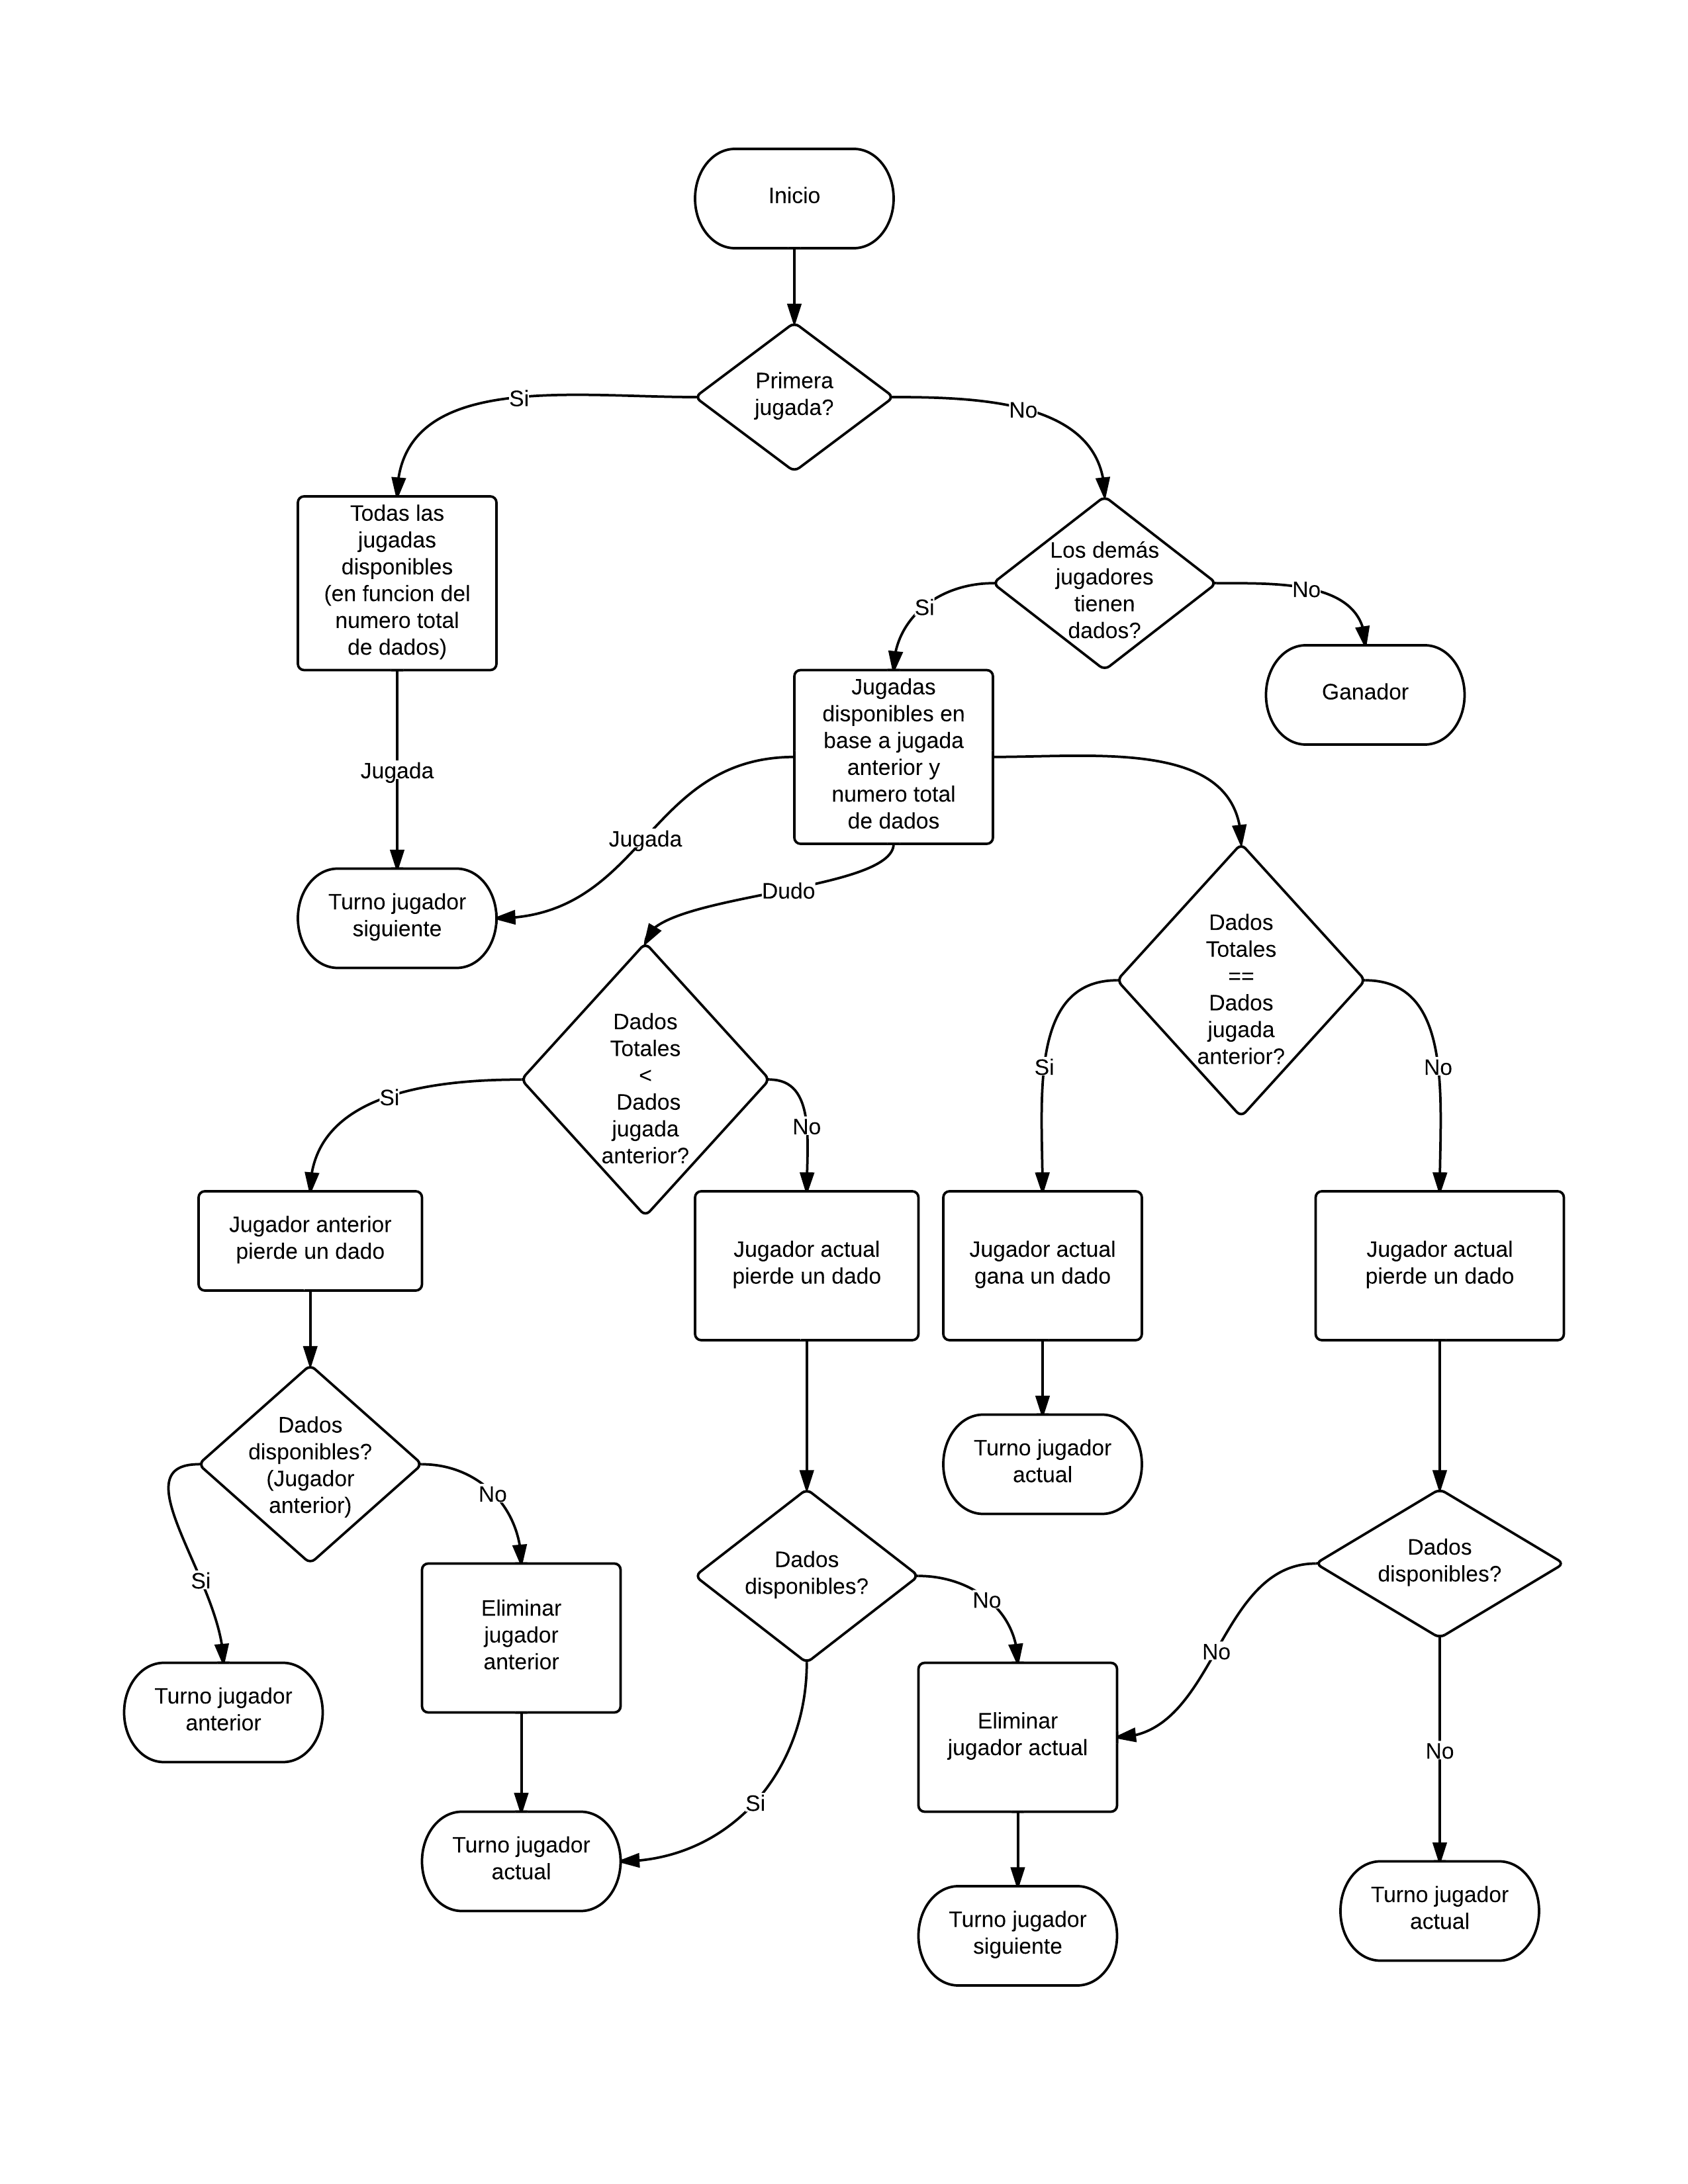
\includegraphics[width=\textwidth]{FlujoDudo.png}
\end{figure}

\newpage
\begin{figure}[h!]
	\centering
		\caption{Modelo de datos}
	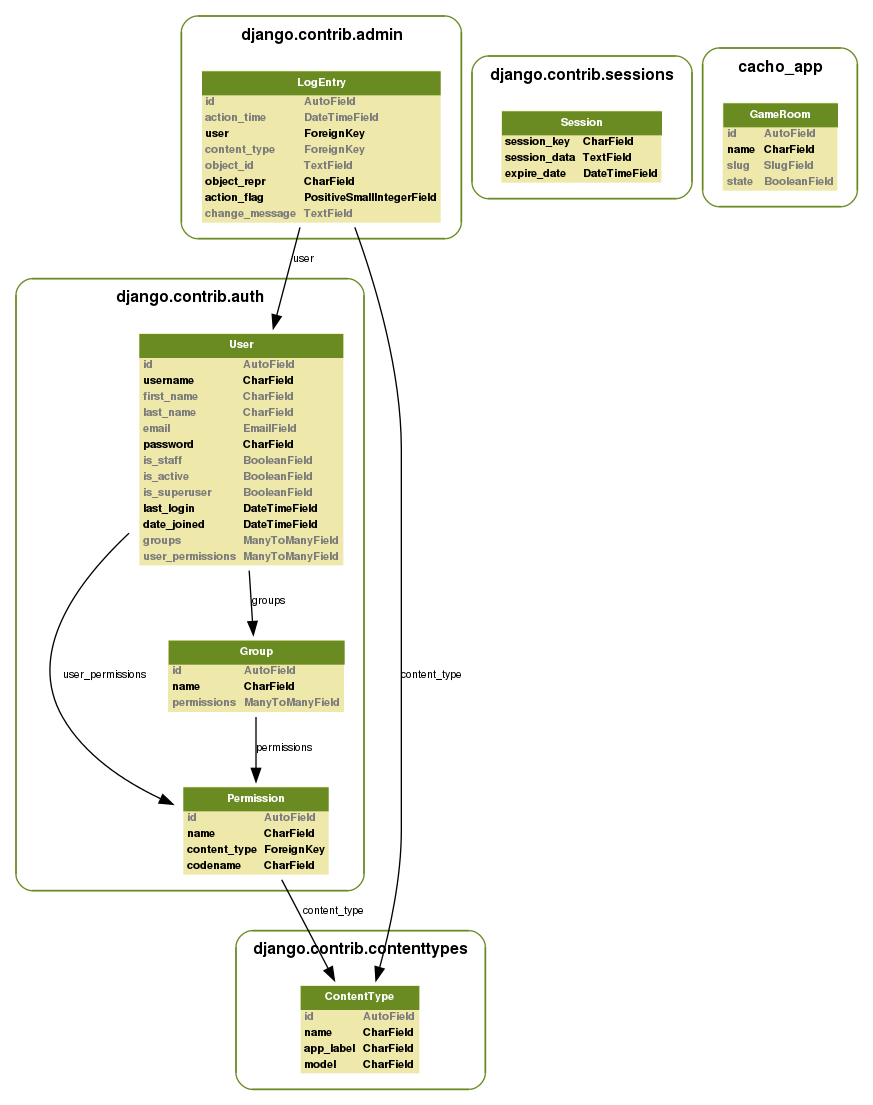
\includegraphics[width=\textwidth]{md.png}
\end{figure}


\newpage
\section{Referencias}
\begin{enumerate}
	\item Documentación oficial de Django -- https://docs.djangoproject.com/en/1.4/
	\item Documentacion de Python -- http://docs.python.org
	\item gevent-socketio API docs. -- https://gevent-socketio.readthedocs.org/
	\item Socket.IO recipes -- https://github.com/LearnBoost/socket.io
	\item Developing Django apps with zc.buildout -- http://jacobian.org/writing/django-apps-with-buildout/
	\item Evented Django -- http://codysoyland.com/2011/feb/6/evented-django-part-one-socketio-and-gevent/
	\item IRC, \#django y \#python en irc.freenode.net
\end{enumerate}

\end{document}


